%% This is file `elsarticle-template-2-harv.tex',
%%
%% Copyright 2009 Elsevier Ltd
%%
%% This file is part of the 'Elsarticle Bundle'.
%% ---------------------------------------------
%%
%% It may be distributed under the conditions of the LaTeX Project Public
%% License, either version 1.2 of this license or (at your option) any
%% later version.  The latest version of this license is in
%%    http://www.latex-project.org/lppl.txt
%% and version 1.2 or later is part of all distributions of LaTeX
%% version 1999/12/01 or later.
%%
%% The list of all files belonging to the 'Elsarticle Bundle' is
%% given in the file `manifest.txt'.
%%
%% Template article for Elsevier's document class `elsarticle'
%% with harvard style bibliographic references
%%
%% $Id: elsarticle-template-2-harv.tex 155 2009-10-08 05:35:05Z rishi $
%% $URL: http://lenova.river-valley.com/svn/elsbst/trunk/elsarticle-template-2-harv.tex $
%%

%%\documentclass[preprint,authoryear,12pt]{elsarticle}

%% Use the option review to obtain double line spacing
%% \documentclass[authoryear,preprint,review,12pt]{elsarticle}

%% Use the options 1p,twocolumn; 3p; 3p,twocolumn; 5p; or 5p,twocolumn
%% for a journal layout:

%% Astronomy & Computing uses 5p
%% \documentclass[final,authoryear,5p,times]{elsarticle}
\documentclass[final,authoryear,5p,times,twocolumn]{elsarticle}

%% if you use PostScript figures in your article
%% use the graphics package for simple commands
%% \usepackage{graphics}
%% or use the graphicx package for more complicated commands
% \usepackage{graphicx}
%% or use the epsfig package if you prefer to use the old commands
%% \usepackage{epsfig}

%% The amssymb package provides various useful mathematical symbols
% \usepackage{amssymb}
\usepackage{gensymb}
%% The amsthm package provides extended theorem environments
%% \usepackage{amsthm}

\usepackage[pdftex,pdfpagemode={UseOutlines},bookmarks,bookmarksopen,colorlinks,linkcolor={blue},citecolor={green},urlcolor={red}]{hyperref}
%% Draft mode for editing
%\usepackage[pdftex,pdfpagemode={UseOutlines},bookmarks,bookmarksopen,colorlinks,linkcolor={blue},citecolor={green},urlcolor={red},draft]{hyperref}

% \usepackage{hypernat}

\usepackage{tikz}
\usetikzlibrary{arrows,calc}
\newcommand{\tikzmark}[1]{%
  \tikz[overlay,remember picture] \node (#1) {};}

\usepackage{breakurl}

\usepackage{listings}

\usepackage{caption}

\lstset{
  basicstyle=\ttfamily,
  showstringspaces=false,
  stringstyle=\color{red},
  morecomment=[l]{/},
  commentstyle=\color{blue},
}

%% The lineno packages adds line numbers. Start line numbering with
%% \begin{linenumbers}, end it with \end{linenumbers}. Or switch it on
%% for the whole article with \linenumbers after \end{frontmatter}.
%% \usepackage{lineno}

%% natbib.sty is loaded by default. However, natbib options can be
%% provided with \biboptions{...} command. Following options are
%% valid:

%%   round  -  round parentheses are used (default)
%%   square -  square brackets are used   [option]
%%   curly  -  curly braces are used      {option}
%%   angle  -  angle brackets are used    <option>
%%   semicolon  -  multiple citations separated by semi-colon (default)
%%   colon  - same as semicolon, an earlier confusion
%%   comma  -  separated by comma
%%   authoryear - selects author-year citations (default)
%%   numbers-  selects numerical citations
%%   super  -  numerical citations as superscripts
%%   sort   -  sorts multiple citations according to order in ref. list
%%   sort&compress   -  like sort, but also compresses numerical citations
%%   compress - compresses without sorting
%%   longnamesfirst  -  makes first citation full author list
%%
%% \biboptions{longnamesfirst,comma}

% \biboptions{}

\journal{Astronomy \& Computing}

%% Upright single quotes in verbatim fields make FITS header examples
%% much more readable
\usepackage{upquote}

%% For draft use color package to indicate open questions that need
%% clarification
\usepackage{color}

%\defcitealias{2015Jenness}{Paper~II}
%\defcitealias{2014Kitaeff}{Paper~III}

\begin{document}

\begin{frontmatter}

%% Title, authors and addresses

%% use the tnoteref command within \title for footnotes;
%% use the tnotetext command for the associated footnote;
%% use the fnref command within \author or \address for footnotes;
%% use the fntext command for the associated footnote;
%% use the corref command within \author for corresponding author footnotes;
%% use the cortext command for the associated footnote;
%% use the ead command for the email address,
%% and the form \ead[url] for the home page:
%%
%% \title{Title\tnoteref{label1}}
%% \tnotetext[label1]{}
%% \author{Name\corref{cor1}\fnref{label2}}
%% \ead{email address}
%% \ead[url]{home page}
%% \fntext[label2]{}
%% \cortext[cor1]{}
%% \address{Address\fnref{label3}}
%% \fntext[label3]{}

\title{The Calibration Reference Data System}

%% use optional labels to link authors explicitly to addresses:
%% \author[label1,label2]{<author name>}
%% \address[label1]{<address>}
%% \address[label2]{<address>}


\author[stsci]{Perry~Greenfield}
\ead{perry@stsci.edu}
\author[stsci]{J.~Miller}

\cortext[cor1]{Corresponding author}
\address[stsci]{Space Telescope Science Institute, 3700 San Martin Drive, Baltimore, MD 21218, USA}

\begin{abstract}
%% Text of abstract

We describe a software architecture and implementation for using rules to
determine which calibration files are appropriate for use in calibrating a
given observation. This new system replaces what had been previously used for
the Hubble Space Telescope (HST) calibration pipelines, a system called the
Calibration Database System (CDBS), and will be used for the James Webb Space
Telescope (JWST) calibration pipelines, and is currently being used for HST calibration pipelines. . The approach used for this can be
easily generalized for use in similar applications that need a rules-based
system for selecting the appropriate file for a given case; we give some
examples of such generalizations that will likely be used for JWST. The core
functionality of the Calibration Reference Data System is available under an
Open Source license.
\end{abstract}

\begin{keyword}
%% keywords here, in the form: keyword \sep keyword

%% MSC codes here, in the form: \MSC code \sep code
%% or \MSC[2008] code \sep code (2000 is the default)

FITS \sep
File formats \sep
Standards \sep
World Coordinate System

\end{keyword}

\end{frontmatter}


% \newcommand{\ascl}[1]{\href{http://www.ascl.net/#1}{ascl:#1}}
\newcommand{\aspconf}{ASP Conf.\ Ser}
\newcommand{\aap}{A\&A}
\newcommand{\aaps}{A\&AS}
\newcommand{\jrasc}{JRASC}
\newcommand{\qjras}{QJRAS}
\newcommand{\mnras}{MNRAS}
\newcommand{\pasp}{PASP}
\newcommand{\pasa}{PASA}
\newcommand{\apjs}{ApJS}

%% main text
\section{Introduction}

When running automatic calibration pipelines one important capability needed is
the ability to identify automatically the appropriate calibration files that
should be used when calibrating the data. The kinds of calibration files are
typically numerous, and there may be many that have to be applied to a specific
dataset. Examples are dark current, bias, flat field, photometric, and
geometric distortions, among many others. Typically calibration files depend on
particular observing modes or parameters, or may be time variable.
Calibration files also differ across instruments both in purpose and specific 
instantiations of a particular reference type.

\section{Prior Solution}

The system that was used for the Hubble Space Telescope (HST) was called the
Calibration Database System (CDBS,  
\citealt{1994Cox,1997Lubow,1998Cox,1997hstinternal,2004Swam}). It was used successfully for many years (with some design changes documented in the 
cited references). The experience with it revealed that there were some limitations that
proved to constrain its capabilities, and as a result, a newer system that
removed these constraints was sought. We will briefly describe the design of
CDBS at a high level and the constraints that it posed. This provides the
necessary background for discussing the design goals of CRDS.

The basic design of CDBS was centered around a database that contained
information on each reference file (the generic STScI term for files used to
calibrate data whether they be flat fields, darks, or file containing
appropriate parameters to use in calibration). Typically the database contained
information about the relevant observational parameters (mostly instrument mode
settings and date of applicability). At the highest level, the basic approach
was to run a program for each new dataset being processed (or reprocessed as
the case may be) that essentially performed a query on the database for each
type of reference file needed. The result of the query was a specific reference
filename that would then be set as the value of a particular keyword in the
dataset's header for use by the calibration pipeline.

The calibration pipelines retrieved the names of the appropriate reference
files from the dataset's header, and used those to open that reference file
for use in calibration. The reference files were kept in a standard location in
the pipeline processing system. The program that updated the headers with the
selected references files was called ``bestref.''

In reality, there was much more to CDBS than what has been briefly
described. The system handled the addition of new reference files, first by
validating the files met certain requirements, and then the archiving of those
submitted files. The process for submitting new files involved a good number of
manual steps and checks. One goal of the replacement system was to streamline
the submission process somewhat.

The most critical aspect of the validation requirements for reference files
concerned the keyword values used to match datasets to the appropriate
references.  Unlike dataset parameter keywords which describe a specific
instrument configuration for one observation, reference file keywords
circumscribe range of parameter values for which the reference applies.  In
CDBS, ranges of parameter values were often represented by intermediate values
which expand into the discrete values used to define specific instrument
configurations.  As part of submitting reference files, the intermediate values
were combinatorially exploded into database rows which represented each
possible application of a reference to some discrete instrument parameter
configuration.  As an example, a dataset APERTURE keyword would describe the
specific aperture an instrument was configured to use for one observation. In
contrast, the same APERTURE keyword specified in a reference file would
describe, indirectly, the combined set of different specific APERTUREs that
reference file was capable of supporting.  When multiple parameters were used
to match datasets to references, the number of distinct rows in the CDBS
database was equal to the product of the number of specific values supported by
a particular reference for each parameter.

Furthermore, there were occasions for which standard SQL queries were
insufficient for achieving the desired selection results. In such cases,
software was run to generate custom queries to get around such limitations.

CDBS was used for 24 years of HST's operation. During that period, upgrades and
enhancements were made to how it worked, but for the most part, the design did
not change in any major way.

\section{Limitations in CDBS}

Twenty four years provides a long time to learn about what could be
improved. This section highlights what issues proved the most problematic in
using CDBS.

\begin{enumerate}
\item Difficulty testing new reference files. The use of a database essentially
limited the system to one set of rules for selecting reference files. Once a
reference file was delivered to the system, effectively the rules for selection
were modified in the operation system immediately. There were occasions when
reference files were deemed to have passed functional testing (i.e., they
performed the correct calibration for the designated cases), but were submitted
with incorrect information about which modes or dates that they should be used
for. As a result, the operational pipeline would only discover that there was a
problem when processing real data, thus resulting in dealing with correcting
mis-processed data (or in some cases, failure to even process). Problems in the
operational pipeline are significant disruptions. In the last few years, a test
version of the database was created so that tests could be performed, but that
introduces synchronization and management issues to make sure what is being
tested corresponds to the previous operational version. Furthermore, if
multiple deliveries are in progress from different instruments, it introduces a
coordination issue to make sure they are either all completed together or in
sequence, which can prove constraining to the needs of each instrument as far
as testing goes.

\item Difficulty in undoing mistakes. A delivery of a file with mistaken
parameters could be difficult to undo. No reference file could be removed from
the database for various reasons. In a number of cases, particularly if the
date that it was targeted for was incorrect, it could seriously corrupt the
selection logic. To take the most common error case: Files often had a
``useafter'' date associated with them that indicated that it should be used for
a date after the specified one *if no other file had a later date that was
still before the date of the observation*. If one submitted a file intended to
be used for data after 2000-01-01 but mistakenly provided
1999-01-01 then two new file submissions are required to correct the problem.
One to resubmit the new file with the correct date; the second to resubmit the file
intended to be used after 1999-01-01 so that its useafter date is one second after
the mistaken submission. 

There are other cases where one mistaken submission may require a series of
resubmissions of already submitted files to correct for the effect of the wrong
submission. One such example is if one mistakenly supplies a``wildcard'' for a
parameter that should only apply to one case. In this event, all the other
reference files intended for each of the other possible parameter values must
be resubmitted. This makes the potential effects of mistakes serious and thus
requires extreme care in submission.

\item Difficulty in supporting remote usage by astronomers. 
Using the bestref facility remotely
requires providing a web service so that remote processing can get the most up
to date recommendations on the best reference file to use. There is one serious
drawback in this though. Frequently the versions of the calibration software in
the operations pipeline have not yet been publicly released, and there are
times when the latest reference files require the latest software. Such a web
service has the potential of recommending reference files that either are
inappropriate for previous versions of the calibration pipeline software, or
simply will not work with previous versions. As a result, this service was not
provided.

\item Difficulty in allowing customized variants of selection rules. Sometimes
observers or teams have specialized calibration files that they wish to
substitute in place of the standard ones. There was no simple way of allowing a
team to run a customized version of CDBS to support this. The entrenched
software requirements were too numerous (when one develops a system to run in
only one environment, dependencies on that environment easily become entrenched
in the system). Even if no customization was desired, it makes running the
calibration pipeline remotely at another institution very difficult since there
is no simple way to get the the most recent recommendations.

\item Difficulty in providing remote pipelines a consistent bestref
environment. There are times observers *do not* want changing references files
if they wish comparison to previously computed results. They want the same
rules applied, even if they aren't the very best version.
As a ``single state'' database expressing only the current best reference
assignment rules, reproducing historical results in CDBS was difficult or
impossible.

\item Difficulty in understanding what the effective rules are. The exact
selection rules are embodied in a database with a history of transactions for
which many supersede previous ones. One really only knows the net effect by
running queries on the database for specific cases, even when something quite
simple could summarize what is desired for the current situation. The net
effect of this is that people do not really understand what the rules are, and
that they are not what was intended. Finding mistakes in this situation can be
quite difficult. And once found, can be difficult to rectify.

\item Difficulty in adding new kinds of selection rules. The database schema
effectively constrains what kinds of rules can be used. More complex rules
either lead to horrendously complex queries, or custom software to generate
custom queries. The use of the custom software/queries ends up making the system
even more opaque.
\end{enumerate}

\section{The Crux of a Different Approach}

It became apparent that many of the limitations ultimately came down to the
dependence on a database as the repository for the selection rules. This has a
number of drawbacks in this particular application:

\begin{enumerate}
\item Databases are effectively one state systems. Yes, one can deal with
multiple states but usually at great complexity.
\item Databases do not make it simple to distribute software since installing,
administering and maintaining a database elsewhere is a major task, and keeping
them synchronized to the master copy is yet a greater complexity
\item Once established, changing the structure of database is difficult,
particularly with a systems used in operations.
\end{enumerate}

Is it in fact necessary to use a database to hold the rules? In reviewing all
the previous and anticipated cases for HST and JWST, it did not appear that a
database was necessary for selection rules, and that a simpler and more
flexible approach could be chosen. Indeed, all that appears to be needed is to
encompass a version of the rules in a simple text file. In doing so there are a
number of immediate benefits:

\begin{enumerate}
\item the rules are explicit
\item multiple versions of these rules may exist without conflict, and used in
different contexts simultaneously without confusion.
\item these rule files may be easily distributed so that remote users can run the
``bestref'' functionality remotely without needing to install or administer
complex software.
\item the rules are easily customized, even by hand if necessary if
users wish to.
\end{enumerate}

\section{High level organization of CRDS}

The software for CRDS can be considered to be in one of three categories:

\begin{enumerate}
\item supporting the bestref functionality
\item supporting submitting new reference files and all the issues that
go with that
\item Supporting format, semantic, and parameter constraint checking for both
references and rules files.  Capability to detect typos, duplicate lines, and
grammatical errors in rules files.   Capability to analyze basic properties
such duplicate or deleted rows,  by pseudo-mode, for supported tables files.
\item providing utilities for making CRDS useful in operations, for instrument
scientists that must generate and monitor reference files, and end users.
\end{enumerate}

Each of these will be described in a separate section. Since most of the design
is centered around the first category, most of the description will be centered
around that.

\section{Bestref Functionality}

\subsection{Design}

The system is centered around rules files that describe (for one version) 
how reference files should be selected for a single type of
reference file. In a general sense, the file consists of a header of sorts that
describes information about what kind of reference file that it is applied to,
what the relevant information from the dataset is needed to make that
selection, and other bookkeeping information. Following that header are the
rules. Generally these are nested sets of criteria that are used to
successively narrow down the selection until a single result is determined. It
is important to understand that there is no intrinsic limit to what structures
can be supported. If more complex cases arise, new structures can be added to
the library to support these. The following lists existing and possible kinds
of selections structures. Those that already are supported are marked with an
`*'. The ones that are not supported are intended to illustrate possible
extensions that are not purely hypothetical. The following examples of files
will illustrate specifically these structures.

\begin{enumerate}
\item matching on sets of discrete parameter values. That is, the item associated
with this specific set of parameters is selected if the parameter values are
matched according to one of several matching approaches. An item may be a file
name, or a nested set of rules that will be evaluated in turn.  
There are a number of different parameter match types, literal, or-glob,
pure regex, between, not, relational, etc.  In the case of multiple parameters,
each parameter is matched across all match cases using a process of elimination
(winnowing) which successively narrows the possible match cases.

\item matching on a sequence of dates. This corresponds to the useafter mechanism
in CDBS. Normally these items will be sorted in date/time order, and the
date/time of the observation is used to select the appropriate item in the list
using a binary search.

\item matching software version requirements. This structure indicates selection
based on versions of the software which item should be selected. It may use
specific versions, or relative (e.g., any version before or up to the specified
version, or any version after the specified version).

\item getting bracketing files. This is useful if some sort of interpolation
between reference files is desired, in which case a pair of results is
returned.

\item matching on ranges of non-discrete values. For example, this may select a
file if an observational parameter is in the specified range. Normally, this
would be a one-dimensional selection, though even more complex multidimensional
volumes could be constructed if need be.
\end{enumerate}

\subsection{Examples}

Figure~\ref{fig:example1} illustrates use of the first two items. Essentially two different configurations are supported, and for each there are three possible choices of reference files that depend on the date of the observation. For example, if the date of the observation for the configuration {\tt (\textquotesingle MIRIFULONG\textquotesingle , \textquotesingle FAST\textquotesingle , \textquotesingle FULL\textquotesingle )} is 2015-04-02, the second choice will be used resulting in the return of {\tt jwst\_miri\_dark\_0032.fits} as the recommended reference file.

\begin{figure*}
\begin{verbatim}
selector = Match({
    ('MIRIFULONG', 'FAST', 'FULL') : UseAfter({
        '2015-01-27 12:05:34' 'jwst_miri_dark_0029.fits',
        '2015-03-22 00:29:01' 'jwst_miri_dark_0032.fits',
        '2015-04-07 09:14:00' 'jwst_miri_dark_0047.fits',
        ...
        }),
    ('MIRIFUSHORT', 'SLOW', 'FULL') : UseAfter({
        '2015-01-25 12:06:34' 'jwst_miri_dark_0099.fits',
        '2015-03-21 00:28:01' 'jwst_miri_dark_0101.fits',
        '2015-04-08 09:13:00' 'jwst_miri_dark_0127.fits',
        ...
        }),
        ...
})
\end{verbatim}
\caption{Example showing basic parameter matching rules coupled with date dependency.}
\label{fig:example1}
\end{figure*}

Figure~\ref{fig:example2} shows the use of the software selection mechanism. In this case if the software version is less than 3.1 (using the typical version semantics) then the first file will be chosen, if less than 5 the second will be chosen, otherwise the last file will be used.

\begin{figure*}
\begin{verbatim}
selector = SelectVersion({
   '<3.1':    'jwst_miri_flat_0065.fits',
   '<5':      'jwst_miri_flat_0073.fits',
   'default': 'jwst_miri_flat_123.fits',
})
\end{verbatim}
\caption{Example showing use of the software version selection mechanism.}
\label{fig:example2}
\end{figure*}

Figure~\ref{fig:example3} shows how two reference files may be selected
that bracket the particular parameter. Here if the parameter has a value 
of 3.2, then the pair of images 
(\texttt{cref\_flatfield\_124.fits}, \texttt{cref\_flatfield\_137.fits}) will be returned

\begin{figure*}
\begin{verbatim}
selector = Bracket({
    1.2: "cref_flatfield_120.fits",
    1.5: "cref_flatfield_124.fits",
    5.0: "cref_flatfield_137.fits",
})
\end{verbatim}
\caption{Example showing bracketing selection.}
\label{fig:example3}
\end{figure*}

Figure~\ref{fig:example4} shows how a
wavelength of 1300 (between 1220 and 1530) results in the partial match 
of \texttt{hst\_wfc3\_flatfile\_0027.fits} and eliminates 
\texttt{hst\_wfc3\_flatfile\_0028.fits}
of as a candidate.   Since \texttt{BETWEEN}
can be used in an arbitrary Match parameter
slot,  potentially multiple times,  volumes can be described, and also
described in concert with other types of match syntax for other parameters
such as wildcard matching or regular expressions.

\begin{figure*}
\begin{verbatim}
selector = Match({
    ('WFC', 'N/A', 'BETWEEN 1220 1530', 'FR782N') :  "hst_wfc3_flatfile_0027.fits",
    ('WFC', 'N/A', 'BETWEEN 1530 1690', 'FR782N') :  "hst_wfc3_flatfile_0028.fits",
    ...
})
\end{verbatim}
\caption{An example showing matching specified ranges.}
\label{fig:example4}
\end{figure*}

[xxx need headers included and explained since examples have unnamed
parameters that won't make any sense unless put in context]

[xxx insert full description of syntax used]

[xxx somewhere put in explanation of safety features preventing hand
mangling of rules files and configuration]

Full documentation of the syntax and semantics of all the rmap and
context files is available on the web 
\footnote{\texttt{https://jwst-crds.stsci.edu/static/users\_guide/rmap\_syntax.html\#selectors}}

\subsection{Hierarchical Organization}

The system is based on these files (which we refer to rmap files since they
indicate the mapping to reference files) but also involves a hierarchy of
related files that are called context files, which provide a nested 
organizational structure corresponding to the functions at different levels. Essentially context files are
text files that define a set of related files that are to be used for
that configuration.
Instrument context files collect all the rmap files for that
instrument. This file effectively defines the versions of all the rmap files
for each reference file types that comprise the version of recommendations in
effect for that instrument. In the example of the instrument context file
below, one can see that each distinct rmap file has a unique name. If anything
is changed in an rmap file, it gets a new name

[xxx need example of instrument context file]

Likewise, there is a pipeline context file that lists the instrument context
files that define the versions in effect for the pipeline being run. As with
rmap files, instrument context files all have unique names. Any change of
content results in a new name for an instrument context file. Finally, the same
is true for pipeline context files. The net result is that a pipeline context
file deterministically identifies all the rules in use for a pipeline. 

Note that one can run any number of pipeline environments, and each may use a
completely different pipeline context if need be, each of which will have some
sort of different rules for how reference files are selected.

[xxx need example of pipeline context file]

This hierarchy is designed to match that for JWST and as such is currently
designed around the current levels of hierarchy. It is a possible generalization
that would allow it to deal with arbitrary levels of heirarchy, perhaps
different in number depending on the branch taken. Achieving that would
take significant modifications but is possible. 

\subsection{Practicality and Restrictions of this design}

This approach assumes that the number of matching rules is reasonable for a
text file (e.g., fewer than 10,000 lines or so). It also assumes that the
number of versions of such files is reasonably bound (again, not more than a
few thousand). The most likely driver for the number of rules files versions is
the addition or modification of new reference files as a function of time. This has
been the case for HST, where it is not uncommon to generate new dark files for
every day. For a mission that may last a decade or more we are looking at
approximately 3-4 thousand if updated daily. In fact, HST updates the
configuration more infrequently (e.g., once a week even if there is a reference
file for each day).

In cases where updates are much more frequent, and the system that uses
them must be reconfigured after each update, CRDS may not be practical. This
may be the case where new calibration files are obtained every few minutes and
automatically turned into reference files for immediate use by a calibration
pipeline.

\subsection{Language independence}

This implementation has been done completely in Python. Although the rmap files
have a Python flavor to them (arguably it is more of a JSON flavor), nothing
requires this functionality to be performed in Python. To date Python has
proven fast enough to generate the bestref functionality, even for recomputing it
for large numbers of exposures, as is needed to determine which datasets must
be reprocessed as a result of changes to the configuration.

\section{Adding and updating reference files, rmaps and contexts}

While the design of the system is very much centered around how reference file
recommendations are made, that is hardly the only important aspect of the
system. How does one submit new files and ensure the integrity of the system as
the content evolves?

One of the important goals for CRDS was to streamline the process of submitting
new files while ensuring that files are well checked before committed, at least
for common use cases for new Reference files. A completely manual approach is
outlined here before addressing more automatic schemes. For the time being, the
details of how files are actually submitted is deferred to the next section

Supposing one or more new references files of a specific type for a specific
instrument are ready to be tested and used in the operations system/:

\begin{enumerate}
\item submit each of the reference files (with validation of each file
being part of the submission process). This is expected to generate
unique names for each of the submitted reference files
\item edit the rmap for that reference file type to include the necessary
changes to use these (most likely either a replacement of older versions
or the addition of time-variable ones).
\item submit the updated rmap file (again with implied validation for
correctness)
and again, generating a new, unique rmap file name that represents the version
of the file in the system that has the desired changes.
\item edit the instrument context file to use the new version of the rmap file.
\item submit the updated instrument context file (with validation and 
generating a new, unique name)
\item edit the pipeline context file to use the new version of the
instrument context file.
\item submit the updated pipeline context file (with validation and 
generating a new, unique name)
\end{enumerate}

At this point the new reference files can be used in an operational
context. Normally, it is expected that they will be tested on a test version of
the operations system by at least running the standard regression test suite
using the new configuration, perhaps with specific tests for the purpose of
testing the new reference files in use. These tests can be performed simply by
specifying a different pipeline context than the one currently being used in
operations, and without impacting the operations behavior.

When tests have been suitably passed, then the operations system can be updated
to use the new context. Should tests indicate that the new context has
problems, it can simply be ignored and never used. Presumably corrections will
be made to the reference files and the corresponding rules to generate a new,
correct context. However, if changes are made to the CRDS software itself,
something that happens frequently in its early stage of development and use,
it does require a separate test system to test updates to CRDS. Currently, 
deliveries always use the test environment, though it is expected that when
software updates are infrequent, the above model will be used for pure
reference file deliveries.

Since any number of context can exist, one can have several in testing
simultaneously. If that is the case, one still needs to be careful in
determining if different contexts need merging of information (as could happen
if different instruments are submitting new files independently).

For JWST, most instances of merging will be as simple as generating a
pipeline context that uses the appropriate instrument context (the items
most likely to be different; i.e., it is not expected that an instrument 
will be merging items at a lower level in the hierarchy).

In any case, if the operations system does end up using an incorrect pipeline
context, reversion to a previously good one is quite simple (something that
could be quite tricky in CDBS).

In the context of HST (see section xxx), reversion to prior sets of 
rules has been used to
support pipeline regression testing and coordinate CRDS with available
historical system states of the rest of the pipeline.

\subsection{Streamlined updates}

While this multi-step update process may be necessary in more complex cases, the
great majority of reference file submissions fall into one of two categories:
1) the replacement of existing references files (e.g., a better flat field) or
the addition of a reference file for a previously unsupported mode; or 2) the
addition of time-dependent references files to address data for specific time
ranges.

In either of these cases, it is quite useful to streamline the process to
effectively make it one step. Namely by the fact of submitting the reference
files, automatically updating and submitting the appropriate rmap to use it,
and in turn, making the corresponding updates and submissions to the context
files. As a result of these submissions, the user then is given all the
relevant names for the new reference files, rmap, and context files, most
importantly the pipeline context file. For this to work properly, the user must
indicate which pipeline context they are basing the changes on. Normally this
is the last one,  known as the ``edit context'' which can be modified several
times in advance of adopting the context as operational in the pipeline.  

There are several other options as well: 

\begin{itemize}
\item operational
\item one of last 10
\item user specified.  
\end{itemize}

Usually only the ``edit context'' is used, but the other choices
enable branching from a common ancestor.  Other activities which are
streamlined here are automatic file checking of reference and generated rules
files, collection of file metadata, and automatic version-to-version
differencing of the generated rules for inspection by the submitter and
verification that the intended changes have occurred prior to confirming
the submission.  Finally, it includes delivery of the files to the archive.

\subsection{Reference File submission details}

The machinery for submitting reference files is an interactive web-based
system. The ability to submit files or make changes requires user
validation. Figure~\ref{fig:publichome} 
shows a screen shot of the home page of the CRDS
system, which is visible to the public. 

File submission is limited to authenticated users. The home page for
authentic pages is shown in Figure~\ref{fig:authenticatedhome}.
The fully automatic
standard process is dubbed ``Batch Reference Submission'' 
in reference to submission of a pile of files for one instrument,
multiple types,  and automatic certification and rules updates.

Figure~\ref{fig:batchsubmission} shows the starting page for submitting
a batch set of files using the streamlined system.

Figure~\ref{fig:goodsubmissionreview} shows the results of a successfully validated batch  submission request.

Figure~\ref{fig:failedsubmission} shows the results of an unsuccessfully validated batch submission request showing what went wrong.

Figure~\ref{fig:confirmedsubmission} shows the results of a successfully completed submission request.


\begin{figure*}[ht!]
\centering
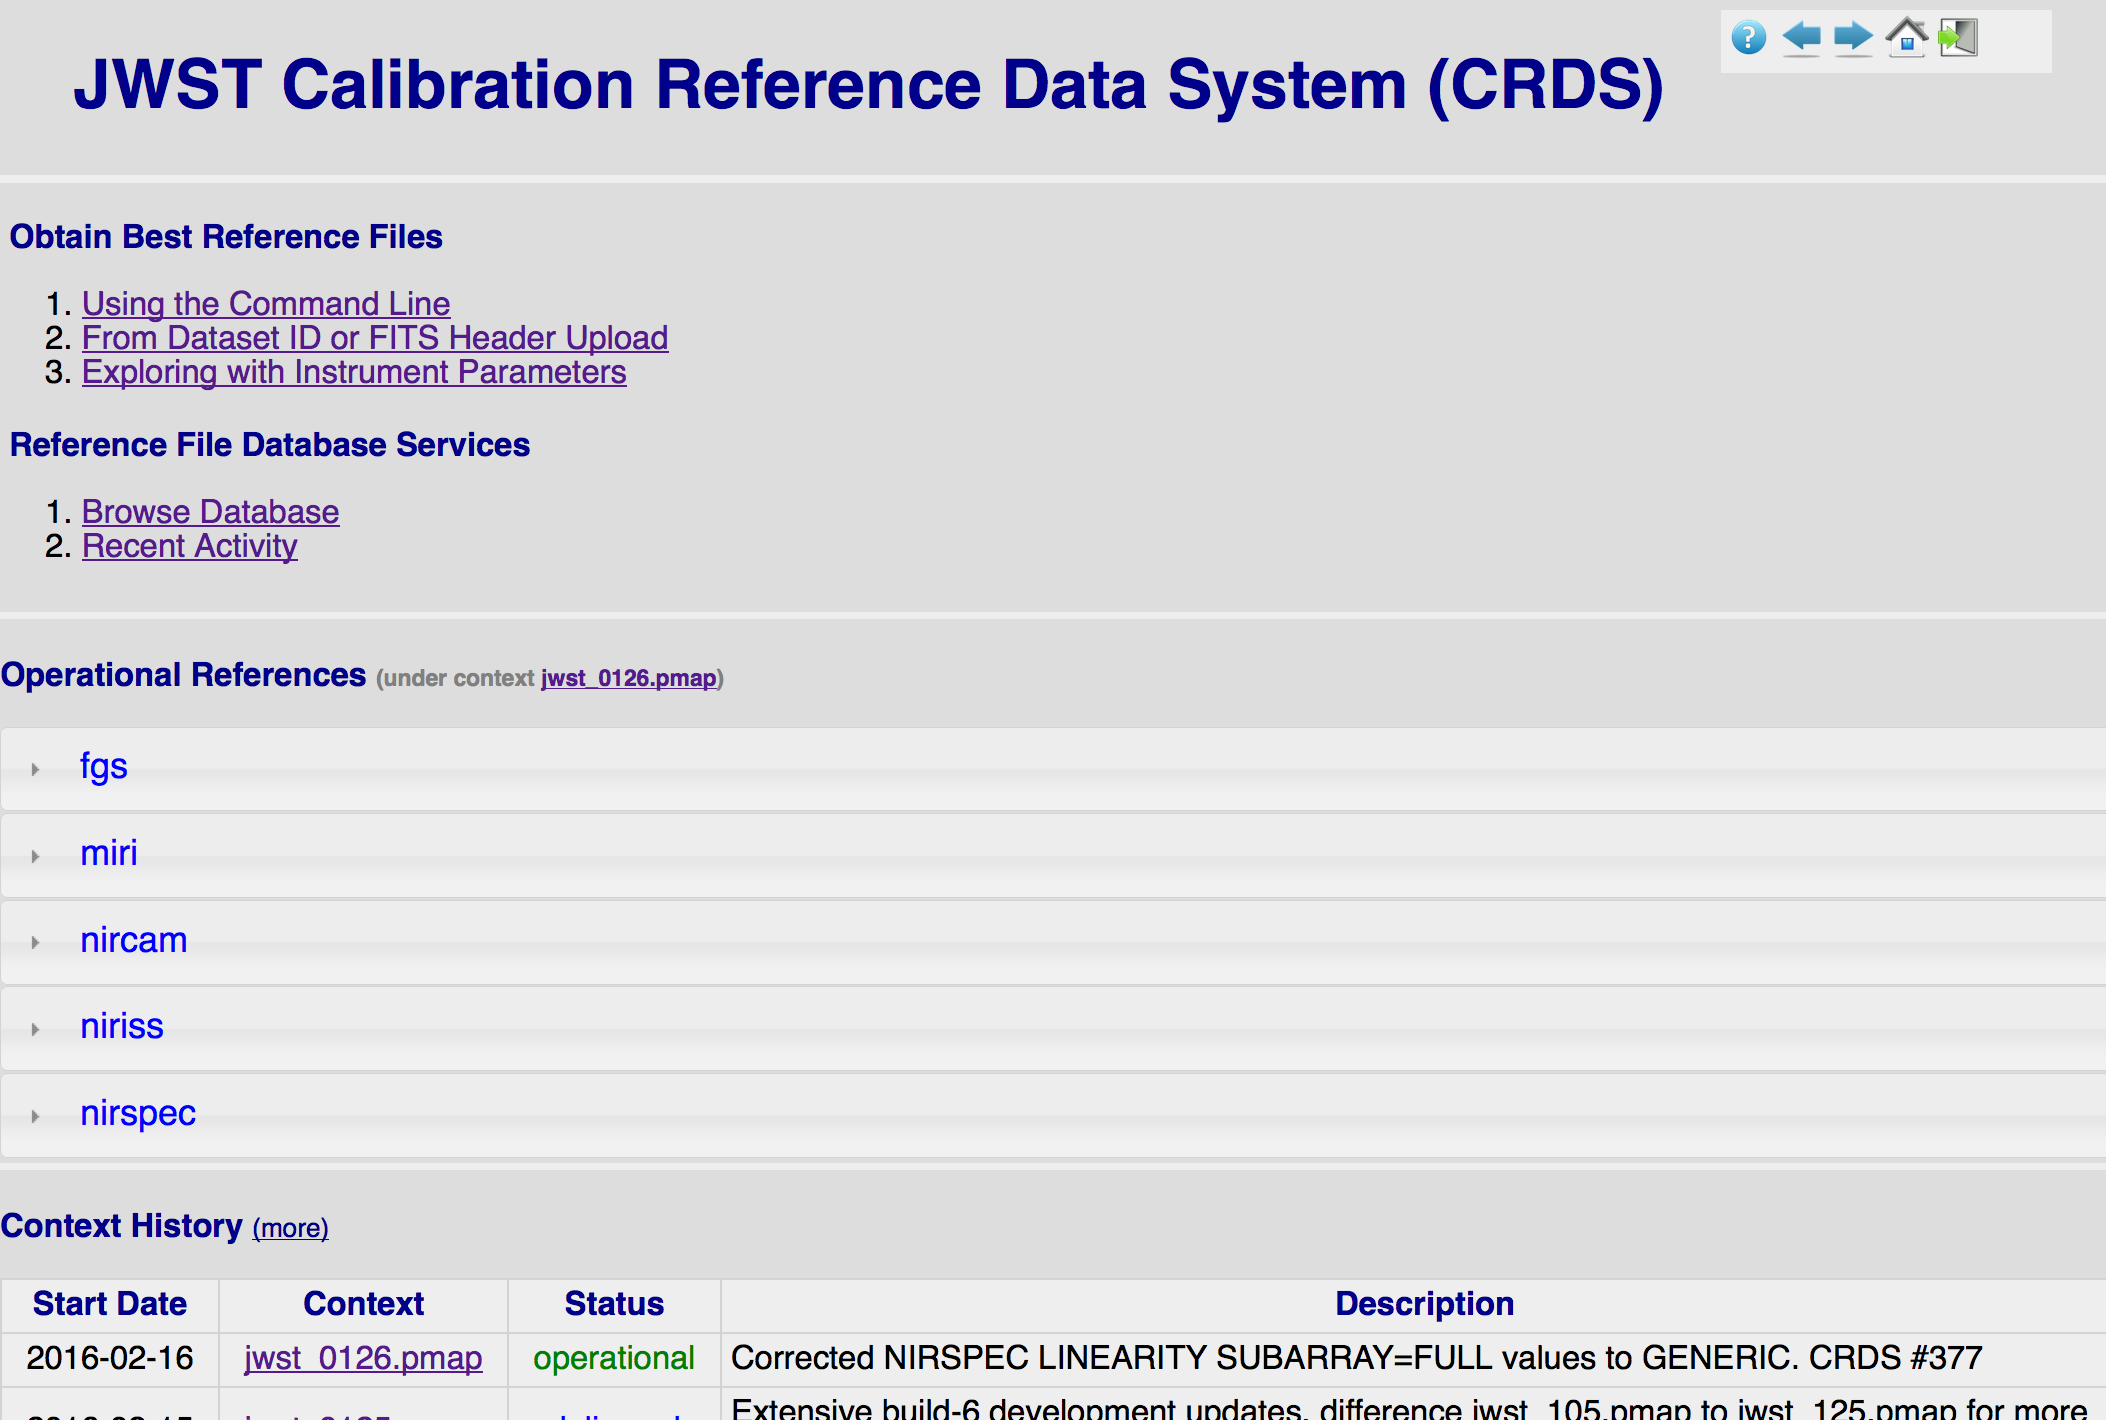
\includegraphics[width=180mm]{JWST_Public_Home_Page.png}
\caption{JWST CRDS Public Home Page}
\label{fig:publichome}
\end{figure*}

\begin{figure*}[ht!]
\centering
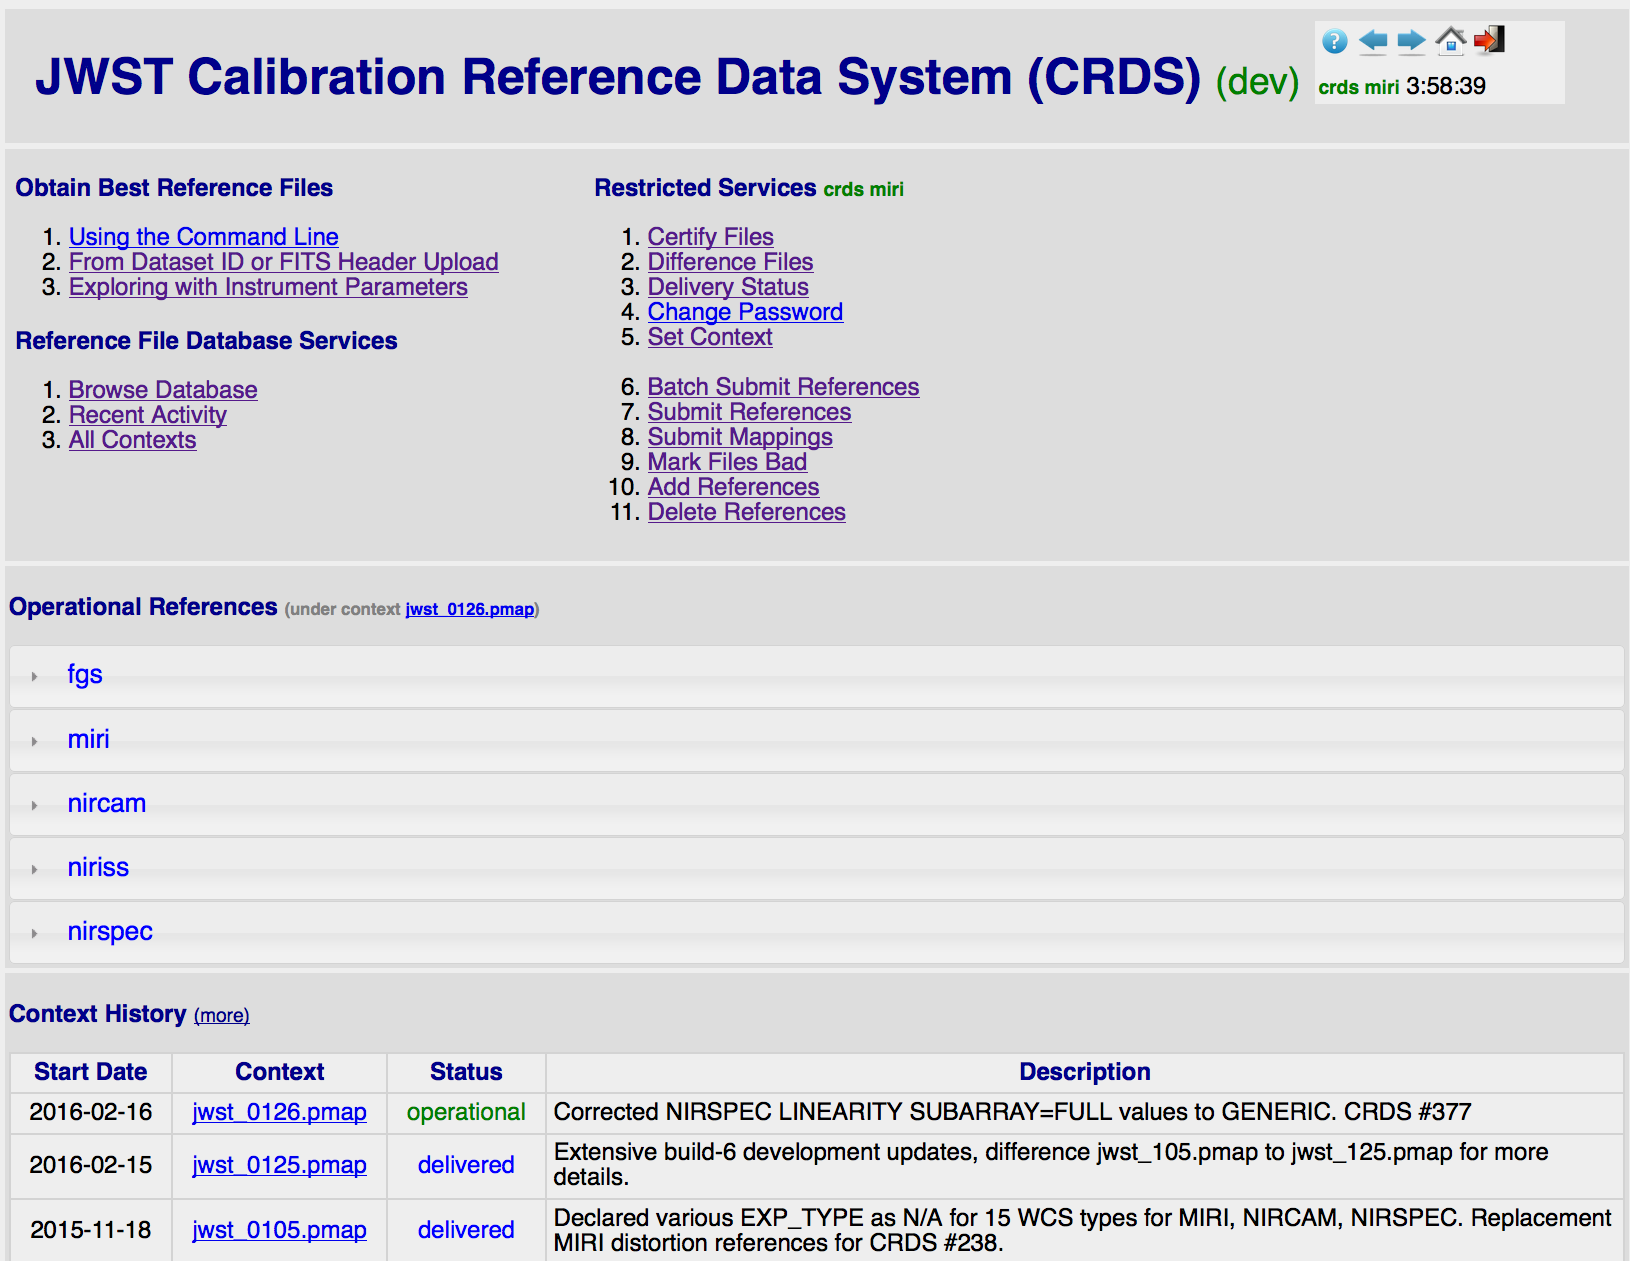
\includegraphics[width=180mm]{JWST_Authenticated_Home.png}
\caption{JWST Authenticated Users Home Page}
\label{fig:authenticatedhome}
\end{figure*}

\begin{figure*}[ht!]
\centering
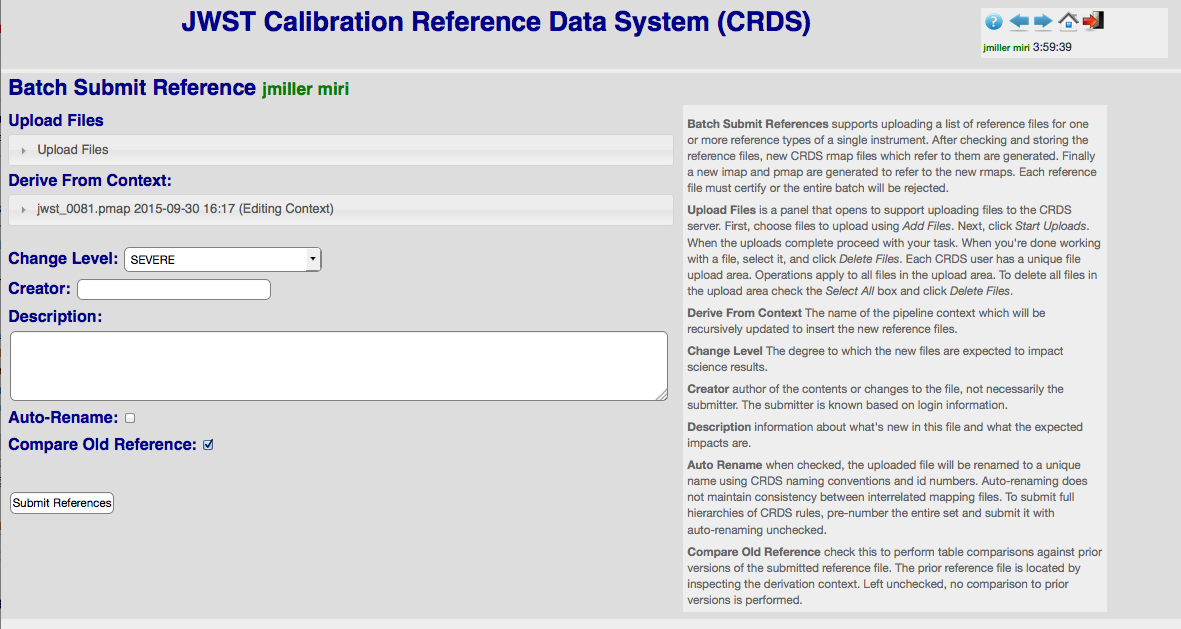
\includegraphics[width=180mm]{JWST_Batch_File_Submission.png}
\caption{JWST Batch File Submission Page}
\label{fig:batchsubmission}
\end{figure*}

\begin{figure*}[ht!]
\centering
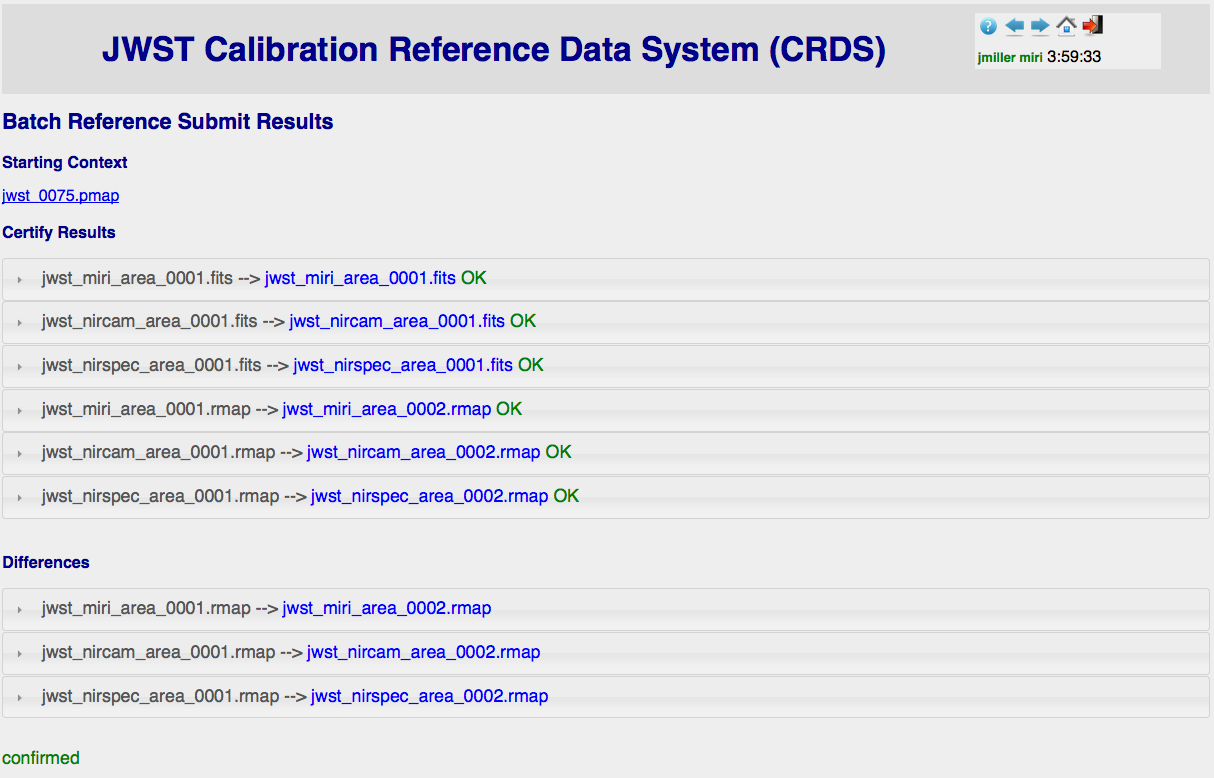
\includegraphics[width=180mm]{JWST_Good_Submission_Review_Page_(after_confirmation).png}
\caption{JWST Good Submission Example}
\label{fig:goodsubmissionreview}
\end{figure*}

\begin{figure*}[ht!]
\centering
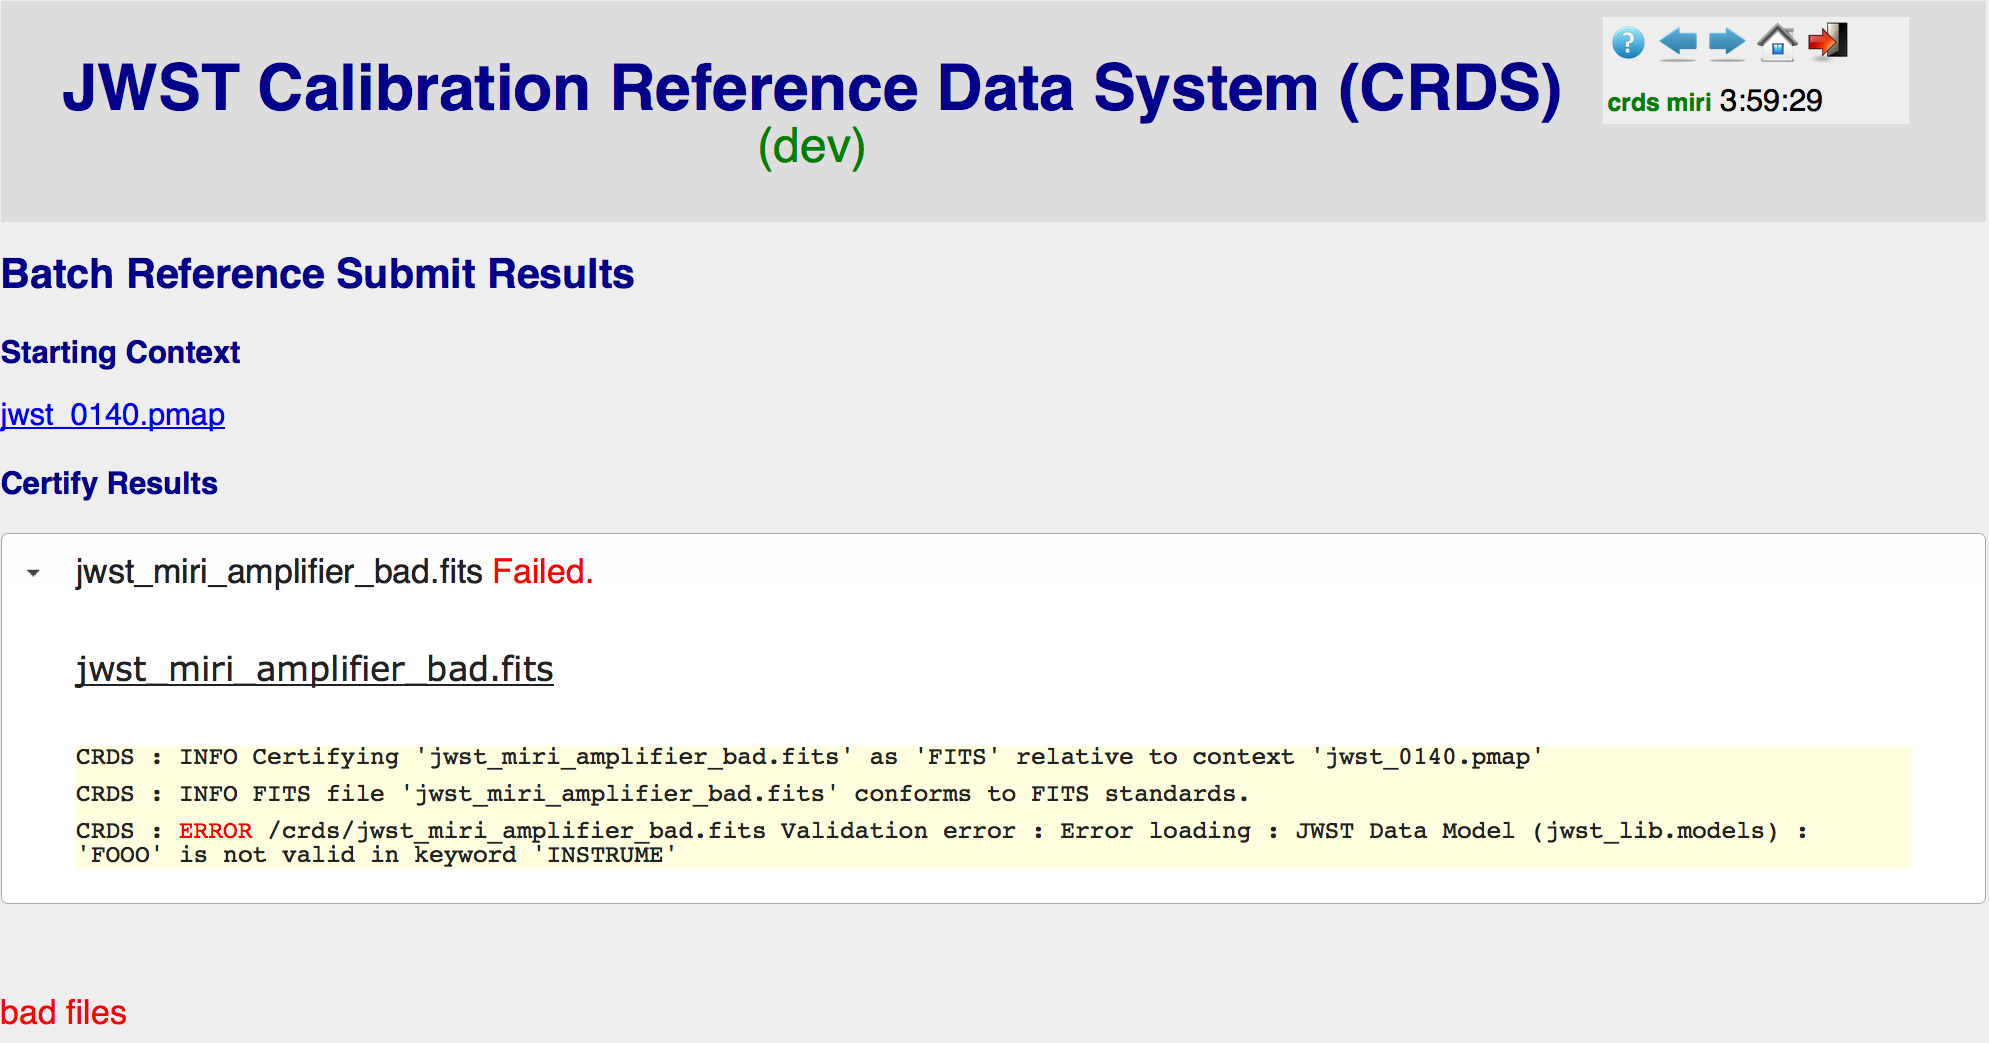
\includegraphics[width=180mm]{JWST_Failed_Submission_DM_schema_violation.png}
\caption{JWST failed submission example}
\label{fig:failedsubmission}
\end{figure*}

\begin{figure*}[ht!]
\centering
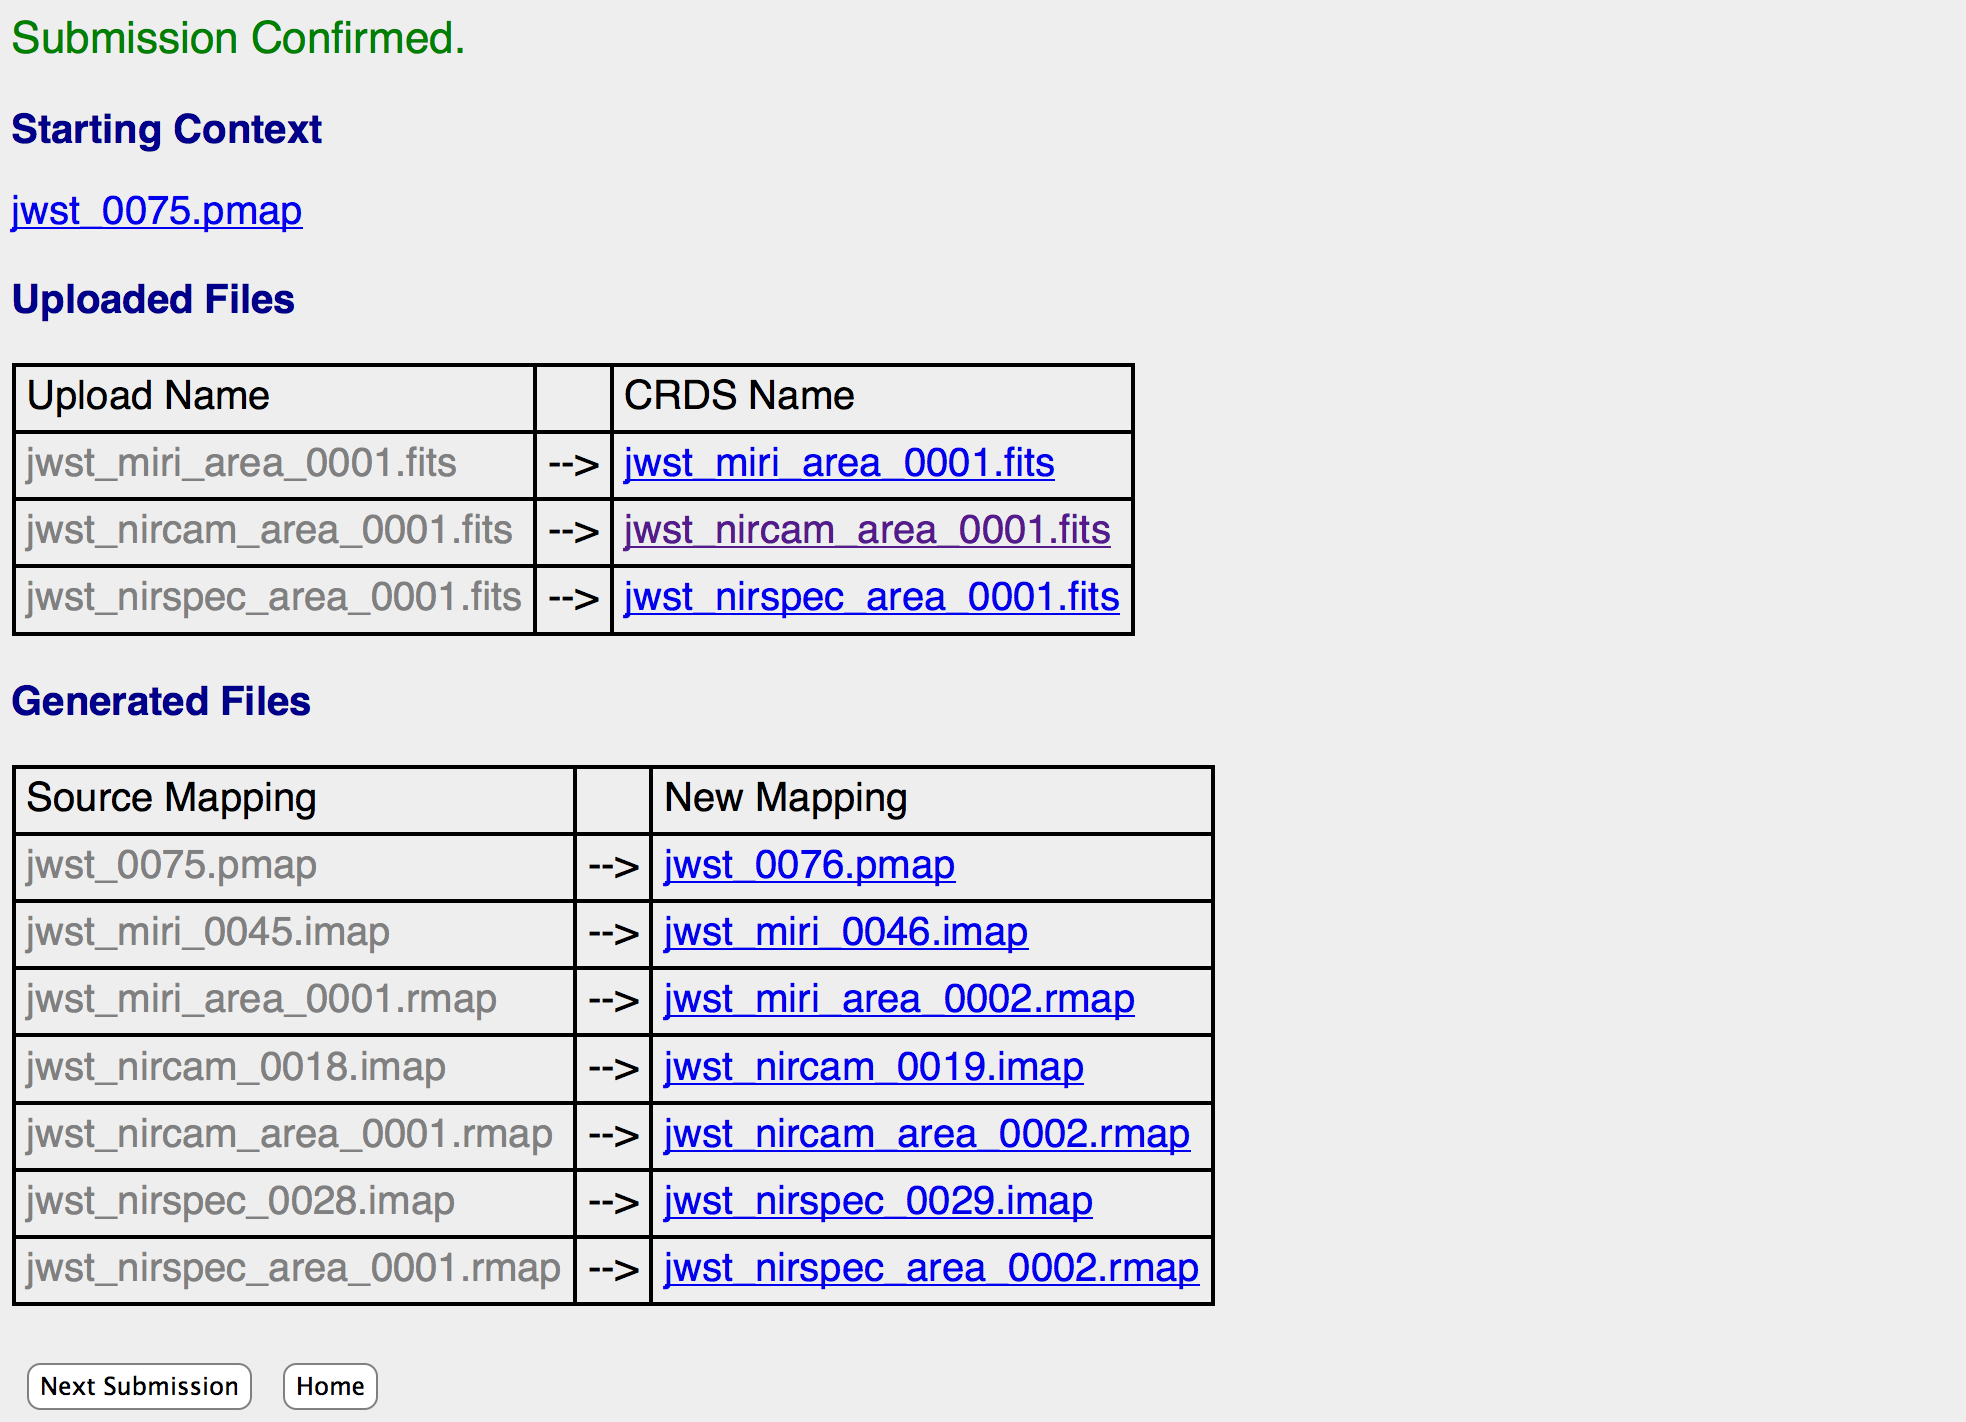
\includegraphics[width=180mm]{JWST_Submission_Confirmed.png}
\caption{JWST submission confirmed example}
\label{fig:confirmedsubmission}
\end{figure*}



The user identifies the local files designated as the files to replace existing
ones. When all the updates have been identified, the submit button [or
whatever] is clicked, and CRDS will then validate each of the reference
files. If they all pass validation, the user will be presented the results of
the results that will be produced (e.g., the new filenames for the reference
files, rmaps and context files, and other summary information). An example of a
successful validation is shown in Figure xxx. At this point the user confirms
the submission after which they will be assigned unique names, added to the
CRDS database of reference files, sent to the STScI archive for archiving, and
placed in the disk-based repository of reference files. If the validation
doesn't pass, the results indicate what the problem is so the user may make the
necessary corrections. Figure xxx shows such a summary of problems.

The subsequent updates to rmap and context files also are validated, primarily
to ensure the syntax is correct.

\subsection{Reference File Validation}

This is handled by using the tools that the JWST pipeline use to validate the
reference files. These are based on data models that use JSON Schema (ref xxx)
to define the mandatory aspects of the data expected, including all the
expected data elements (whether arrays or tables), the allowable dimensionality
and datatype, and required metadata.

The required metadata includes information on who made the reference file, how
the reference file was made and related information (CRDS will also add
standard metadata related to the submission aspects, such as when the file was
submitted.)

There are further checks on file submissions that are intended to warn regarding
suspicious changes. These changes may be valid, but like indicate a mistake. The
following such situations raise a warning on submission:

\begin{enumerate}
\item The reversion of a file to a previous version. For example, 
if a rmap has an
existing reference file name replaced by one that is earlier in the submission
sequence, that would be unusual, and the submitter warned about this reversion.
Likewise if instrument or pipeline contexts point to earlier rmaps or instrument
contexts, respectively, that raises a warning.

\item If someone tries to commit files that were based on a pipeline context that
is no longer the latest, a warning will be raised. By doing so they may reverse
changes made by other instruments that have gotten into contexts after they
started making edits (this normally would not happen with streamlined submission
processes, but only when users are making submissions for individual components
thus raising the possibility they are bypassing subsequent changes).

\item other cases? xxx
\end{enumerate}

\section{Utilities}

Utilities are generally targeted to one or more of three classes of users:
Operations, Instrument Scientists (i.e., those that must create and maintain
reference files), and general users. Some utilities are useful for only one of
these classes of users whereas others may be more broadly useful. We will
organize this section by this class of users. Where a utility has other uses we
will indicate that.

\subsection{Operations}

Affected files utility: Given a list of datasets, determine which ones have
been affected by a change in a pipeline context. Normally it is expected that
the relevant selection parameters for each dataset is contained in a database
to avoid having to examine the contents of each dataset. This utility needs to
run in a reasonable amount of time since it may have to do this comparison for
hundreds of thousands of datasets. The inputs to the utility is a text list of
datasets, and the two pipeline contexts being compared. The results of this
can be used to determine which datasets must be reprocessed to take advantage
of any improved reference files.

Active reference files in a context: List all reference files used in a
pipeline context. This indicates what files may be needed to process the
data. (possibly useful for other classes of users)

\begin{verbatim}
% python -m crds.list --contexts 
     jwst_0059.pmap --references
jwst_fgs_gain_0000.fits
jwst_fgs_gain_0001.fits
jwst_fgs_ipc_0001.fits
jwst_fgs_ipc_0002.fits
jwst_fgs_linearity_0004.fits
jwst_fgs_linearity_0005.fits
jwst_fgs_mask_0002.fits
jwst_fgs_mask_0003.fits
jwst_fgs_readnoise_0000.fits
jwst_fgs_readnoise_0001.fits
...
\end{verbatim}

Inverse mapping: Which rmaps and contexts use a specific reference file (e.g.,
if one finds that one was defective, identify all the pipeline contexts that
used that file so that users may be notified)?

\begin{verbatim}
% python -m crds.uses jwst_fgs_gain_0000.fits
...
jwst_0078.pmap
jwst_0079.pmap
jwst_0080.pmap
...
jwst_fgs_0003.imap
jwst_fgs_0004.imap
jwst_fgs_0005.imap
...
jwst_fgs_gain_0000.rmap
jwst_fgs_gain_0001.rmap
\end{verbatim}

\subsection{Instrument Scientists}

Difference in rules between two contexts: Summarize what has changed in the
rules between two pipeline or instrument contexts. This allows instrument
scientists to quickly identify the changes made.

\begin{verbatim}
% python -m crds.diff jwst_0080.pmap jwst_0081.pmap 
  --brief --squash-tuples
  jwst_miri_regions_0004.rmap 
  jwst_miri_regions_0005.rmap 
  -- MIRIFUSHORT 12 SHORT N/A 
  -- added Match rule for jwst_miri_regions_0006.fits
jwst_miri_0048.imap jwst_miri_0049.imap -- regions -- replaced jwst_miri_regions_0004.rmap with jwst_miri_regions_0005.rmap
jwst_0080.pmap jwst_0081.pmap -- miri -- replaced jwst_miri_0048.imap with jwst_miri_0049.imap
\end{verbatim}

\subsection{General users}

Compare retrieved data with current pipeline context: A user has downloaded
data and wishes to see what data may need to be re-retrieved since the
reference files it used are not the currently recommended ones. A variant on
this is to update the headers of the files with the newly recommended files
(though for the JWST pipelines, this isn't normally necessary). This typically
will be run remotely and thus need network access to the CRDS server.

\section{Technical implementation details}

All the software (aside from a limited amount of web interface tools) is
written in Python. The bestref functionality uses the following Python
libraries (i.e., what isn't part of the Python Standard Library
distribution). It was originally written to use Python 2, but has since been
updated to use Python 3. The server-side libraries have not been ported to 
Python 3 yet.

\subsection{Client side dependencies:}

\begin{itemize}
\item rules file checking uses the **Parsley** parser generator package to define a grammar capable of detecting duplicate lines (cut-and-paste errors)
  \begin{itemize}
  \item jwst\_lib.models, jwst\_lib.stpipe, jwst\_lib.modeling (STScI)
  \item PyYaml
  \item pyasdf (STScI)
  \item astropy
  \item numpy
  \end{itemize}
\end{itemize}

\subsection{Server-side dependencies:}

The web-based functionality uses the Django framework and the MySQL database
backend. The additional following libraries are used.

\begin{itemize}
\item Apache web server using the Python mod\_wsgi as the library interface.
\item django-file-upoad (source code subsumed into CRDS code with modifications):
  Used to  manage parallel file uploads, drag-and-drop, progress bars, data rate info,  remote file deletion,  pause/resume,  etc.)
\item django-locking (source code subsumed into CRDS code with modifications):
  This is database-backed resource locking used to provide ``instrument lock''
   to limit submissions to one person per instrument (to prevent concurrent 
   submissions).
\item django-json-rpc: Supports the interface between the server and clients.
\item django-dbbackup: Used to backup the database and mirror the database between
  different environments
\item pytz: timezone support
\item jQuery/jQuery-UI: web page interface support
\item DataTables: Table display and manipulation for jQuery
\item MochiKit: Javascript debug shell used by django-json-rpc.
\item memcached / libevent / python-memcached: supports cached results on server
\end{itemize}

\section{Limitations and Improvements}

Web uploads are capably (not perfectly) handled by the django-file-upload
system which is fully integrated with the CRDS code base.  An end-to-end
checksum (sha1sum-based) verification of file uploads would be desirable
for extremely large
(DVD-sized) files.  Direct copies to the CRDS server file upload directories
can be used to bypass inefficient (and potentially less reliable) remote
web-based file uploads.

A significant design issue exists with processing and ingesting unbounded
amounts of data in a single file submission and web transaction.  
The primary limitation of large numbers of files and/or high volumes
of data is the time required to copy and compute 
the sha1sum for the file within
the web server.  Each 4G JWST file currently takes on the order of 
2 minutes just to copy or checksum.   This basic data transfer
time dwarfs the timing one would ideally desire for a web response,  
tens of milliseconds, putting CRDS deep into the regime of ``long polling''.    
Because of the current implementation, the web response time is
unbounded and at risk of exceeding proxy timeouts which cancel 
the overall transaction with the web server.   Processing times for 
real world HST file submissions have approached an hour and
in practice have exceeded generous proxy timeout limits.

This can be
mitigated by partitioning files into multiple smaller submissions (also smaller
incremental *failure groups* for certification errors or other problems) or
using alternate backend delivery mechanisms for particularly large submissions.
After initial bootstrappng, all incremental JWST reference updates to date have
been successfully ingested using the web interface.  Fully addressing large
file submissions requires the addition of background processing which isolates
file ingest processing from web protocol timing; this amounts to the addition
of a miniature hidden pipeline in CRDS.  

An additional challenge associated
with the submission of large volumes of data is the loss of processing time
associated with a single errant file forcing the cancellation of the entire
batch.  As the number of files and volume of data in one batch increases, the
processing time increases linearly, and the penalty for errors in submitted
files also increases linearly.  It's bad when file 1199 of 1200 fails wiping
out an entire day of ingest processing.  

Automatically partitioning submissions into reasonable chunks of work is a 
challenging requirement. Because of the unknown semantics and 
interrelationships between the potentially multiple (new or old) types 
in a single submission, human intelligence is required to partition files 
into meaningful groups which can be isolated and used independently 
of other potentially failing groups. However, it is relatively
easy for submission system to warn the user regarding excessively large 
submission requests with suggestions that the submission be partitioned.

Reference files in FITS, JSON, and ASDF format are supported.

\section{Enabling pipeline flexibility}

CRDS was designed to allow running the JWST calibration pipelines remotely much
more easily. HST users could always rerun pipelines at their home institutions,
but it was considerably more painful to do since they had to determine what
reference files their datasets required and retrieve them from the archive
before they could run the pipeline. Even the first task was made more
complicated by the fact that there was no reliable way to find the current best
reference files.

For JWST, CRDS will provide a web service that can be accessed
remotely. Furthermore, the JWST calibration pipelines have been designed to
make the request directly to CRDS to determine which reference files to use and
download the file if it is not available locally. This means anyone can run the
pipeline remotely and be assured that the right reference files will be used,
and retrieved if necessary.

In fact, the bestref functionality has been designed to work entirely locally
if all the necessary context and rmap files are available locally. And the
normal mode of operation is to cache all the files for that functionality even
if running remotely. Once these files are downloaded, the only necessary
internet connection is to check if the context used locally is the current one
being used for JWST operational pipelines. Otherwise, it is entirely possible
to run this functionality entirely locally. The bestref functionality is very
portable and easy to distribute with with the calibration pipeline software.

Another aspect of the pipeline flexibility is that this also allows users to
control the reference file rules. For example, there are cases for which users
prefer to continue using the same reference files as for previous data that has
been calibrated remotely in preference to using slightly better reference
files, but introducing an inconsistency in processing the different data
sets. Users may be able to specify a specific pipeline context instead of the
current context.

Finally, users may edit the rules files directly to replace STScI supplied
reference files with their own ones, or even to add a custom step to the
pipeline with an entirely new set of rules and reference files.

\section{Use for HST}

Although CRDS was designed for use with JWST, it was desired to upgrade the HST
system to use it as well. The advantage for JWST is that CRDS would be heavily
tested in an operational environment. The bestref machinery is essentially
identical, but different in application since HST pipelines populate the data
set's header with the reference files to be used rather than the calibration
pipeline using the service.

The major challenge for HST was in translating the effective rules that existed
in the database into rmap files and ensuring that CRDS was producing the same
results. This was done by doing the recommended comparison for every dataset
in the HST archive. The generation of the rmaps was automated since the target
was constantly changing for HST because of continual reference file
updates. The cycle of generating rmaps and making the reference file comparison
for all datasets was repeated many times until CRDS went operational. This was
further complicate by the fact that the database that contained the CDBS best
references was not reliable. The differences that arose had to be further
tested with the operations bestref facility (which requires using actual
datasets thus is much slower).

This testing uncovered a number of yet undiscovered problems with the CDBS
recommendations, which were then fixed in both.

The two systems were run in parallel for many months with the results being
compared, first with CDBS used for the actual results, then switching to CRDS
as the primary system. CDBS has since been disabled.

\section{Other Applications}

It is important to realize that this system has a wider range of application
than just for selecting appropriate reference files. It can act as a selector
many uses so long as the number of selections is not enormous, and the set of
selection parameter is reasonably consistent and bounded for all data
sets. Other uses are already envisioned for JWST. For example, it will be used
to determine which calibration pipeline to run for the dataset supplied. 
So rather than supplying a reference file to use, it will supply the pipeline 
to execute (either as a name of an executable, or more exactly, a pipeline 
configuration file that the pipeline startup system uses to execute the right
pipeline). It may also be
used to aid in mapping data files to the appropriate data analysis object model
for the data analysis software.

In cases where the parameter sets branch significantly (e.g., when dealing with
data from widely different instruments or even observatories where it is likely
very different conventions are being used for metadata) one may possibly invoke
CRDS tools iteratively, using the first iteration to branch to different sets of
rules on a small subset of the metadata, to cases where each branch has more
consistent metadata.

\section{Licensing and Availability}

The bestref client library has a 3-clause BSD and available through its
repository (xxx). The server side software (e.g., the machinery that handles
file submissions and web services) is not publicly available due to security
concerns, though it is possible that it may be made publicly available once it
has been vetted to be free of any security issues. We will make it available to
qualified institutions and individuals provided that they agree not to make it
publicly available. The client library is quite portable. The server-side
software has more local (STScI) dependencies as well as library dependencies,
and all the configuration, administration , and security issues providing a
server entails.






\section{Acknowledgments}

This work was supported by the JWST mission, a joint effort of NASA,
ESA, and CSA. STScI is operated on behalf of NASA by the Association
of Universities for Research in Astronomy, and by the HST mission xxx
The implementation was aided by
Jonathan Eisenhamer, and the integration into the operations system by Michael
Swam. Testing from the instrument scientist perspective was carried out by Rosa
Diaz and Matthew McMaster. Motivations for the work were provided by the weekly
Science Software Branch Donut meeting.

%% The Appendices part is started with the command \appendix;
%% appendix sections are then done as normal sections
%% \appendix

%% \section{}
%% \label{}

%% References
%%
%% Following citation commands can be used in the body text:
%%
%%  \citet{key}  ==>>  Jones et al. (1990)
%%  \citep{key}  ==>>  (Jones et al., 1990)
%%
%% Multiple citations as normal:
%% \citep{key1,key2}         ==>> (Jones et al., 1990; Smith, 1989)
%%                            or  (Jones et al., 1990, 1991)
%%                            or  (Jones et al., 1990a,b)
%% \cite{key} is the equivalent of \citet{key} in author-year mode
%%
%% Full author lists may be forced with \citet* or \citep*, e.g.
%%   \citep*{key}            ==>> (Jones, Baker, and Williams, 1990)
%%
%% Optional notes as:
%%   \citep[chap. 2]{key}    ==>> (Jones et al., 1990, chap. 2)
%%   \citep[e.g.,][]{key}    ==>> (e.g., Jones et al., 1990)
%%   \citep[see][pg. 34]{key}==>> (see Jones et al., 1990, pg. 34)
%%  (Note: in standard LaTeX, only one note is allowed, after the ref.
%%   Here, one note is like the standard, two make pre- and post-notes.)
%%
%%   \citealt{key}          ==>> Jones et al. 1990
%%   \citealt*{key}         ==>> Jones, Baker, and Williams 1990
%%   \citealp{key}          ==>> Jones et al., 1990
%%   \citealp*{key}         ==>> Jones, Baker, and Williams, 1990
%%
%% Additional citation possibilities
%%   \citeauthor{key}       ==>> Jones et al.
%%   \citeauthor*{key}      ==>> Jones, Baker, and Williams
%%   \citeyear{key}         ==>> 1990
%%   \citeyearpar{key}      ==>> (1990)
%%   \citetext{priv. comm.} ==>> (priv. comm.)
%%   \citenum{key}          ==>> 11 [non-superscripted]
%% Note: full author lists depends on whether the bib style supports them;
%%       if not, the abbreviated list is printed even when full requested.
%%
%% For names like della Robbia at the start of a sentence, use
%%   \Citet{dRob98}         ==>> Della Robbia (1998)
%%   \Citep{dRob98}         ==>> (Della Robbia, 1998)
%%   \Citeauthor{dRob98}    ==>> Della Robbia


%% References with bibTeX database:

\makeatletter
    \clubpenalty10000
    \@clubpenalty \clubpenalty
    \widowpenalty10000
\makeatother

\bibliographystyle{model2-names}
\bibliography{asdf}

%% Authors are advised to submit their bibtex database files. They are
%% requested to list a bibtex style file in the manuscript if they do
%% not want to use model2-names.bst.

%% References without bibTeX database:

% \begin{thebibliography}{00}

%% \bibitem must have one of the following forms:
%%   \bibitem[Jones et al.(1990)]{key}...
%%   \bibitem[Jones et al.(1990)Jones, Baker, and Williams]{key}...
%%   \bibitem[Jones et al., 1990]{key}...
%%   \bibitem[\protect\citeauthoryear{Jones, Baker, and Williams}{Jones
%%       et al.}{1990}]{key}...
%%   \bibitem[\protect\citeauthoryear{Jones et al.}{1990}]{key}...
%%   \bibitem[\protect\astroncite{Jones et al.}{1990}]{key}...
%%   \bibitem[\protect\citename{Jones et al., }1990]{key}...
%%   \harvarditem[Jones et al.]{Jones, Baker, and Williams}{1990}{key}...
%%

% \bibitem[ ()]{}

% \end{thebibliography}

\end{document}

%%
%% End of file `elsarticle-template-2-harv.tex'.
